\documentclass[a4paper,11pt,twoside]{article}
%\documentclass[a4paper,11pt,twoside,se]{article}

\usepackage{UmUStudentReport}
\usepackage{verbatim}   % Multi-line comments using \begin{comment}
\usepackage{courier}    % Nicer fonts are used. (not necessary)
\usepackage{pslatex}    % Also nicer fonts. (not necessary)
\usepackage[pdftex]{graphicx}   % allows including pdf figures
%\usepackage{lmodern}   % Optional fonts. (not necessary)
%\usepackage{tabularx}
%\usepackage{microtype} % Provides some typographic improvements over default settings
%\usepackage{placeins}  % For aligning images with \FloatBarrier
%\usepackage{booktabs}  % For nice-looking tables
%\usepackage{titlesec}  % More granular control of sections.

% DOCUMENT INFO
% =============
\department{Institution för Datavetenskap}
\coursename{Datavetenskapens byggstenar 7.5 p}
\coursecode{DV160HT15}
\title{OU3 Tables}
\author{Lorenz Gerber  ({\tt{dv15lgr@cs.umu.se}})}
\date{2015-12-17}
%\revisiondate{2015-09-15}
\instructor{Lena Kallin Westin / Johan Eliasson}


% DOCUMENT SETTINGS
% =================
\bibliographystyle{plain}
%\bibliographystyle{ieee}
\pagestyle{fancy}
\raggedbottom
\setcounter{secnumdepth}{2}
\setcounter{tocdepth}{2}
%\graphicspath{{images/}}   %Path for images

% DEFINES
% =======
%\newcommand{\mycommand}{<latex code>}


% DOCUMENT
% ========
\begin{document}
\maketitle

\tableofcontents
\newpage

\section{Introduction} 
The aim with this laboration was to understand and a set of given 
composite data types and then built on those implement two new ones.
Test code for correctness and speed was given. The given datatypes
were directed `list', `array', and a `table', implemented using the 
aforementioned directed list. The used programming language was `C'. 
The datatypes to be implemented were table using a `move-to-front 
list' and `table' using `array'.

The implementation of the datatype `table' is according to the 
defintion in the coursebook \cite[pp. 117 -- 132]{janlert2000}. In Brief:
a `table' is a finite mapping of arguments to values. The textbook states 
a dictionary as a model where the lookup words are the arguments and the
textual explanations the values. The datatype `table' however, does not 
need to be ordered by definition.

The operations found in the interface of a table are `empty', to create
an new empty `table', `insert' to put new argument, value pairs into an 
exisiting `table', `isEmpty' to check whether an existing `table' has any
content, `lookup' to access the value associated to a potentially available
argument in an existing table and `remove' to discard a potentially
existing argument/value pair from a existing table.  

The assigment included also testing and benchmarking of both the given and
the requested table implementations. The benchmarking was ment to
allow discussing the different implementations from a number of different
aspects such as lookup speed of existing and non-existing arguments, insertion
and removal speed as well as skewed or biased lookup. As a starting point,
number of mandatory questions and discussion topics were given in the
lab instructions.  

\begin{figure}[H]
\centering
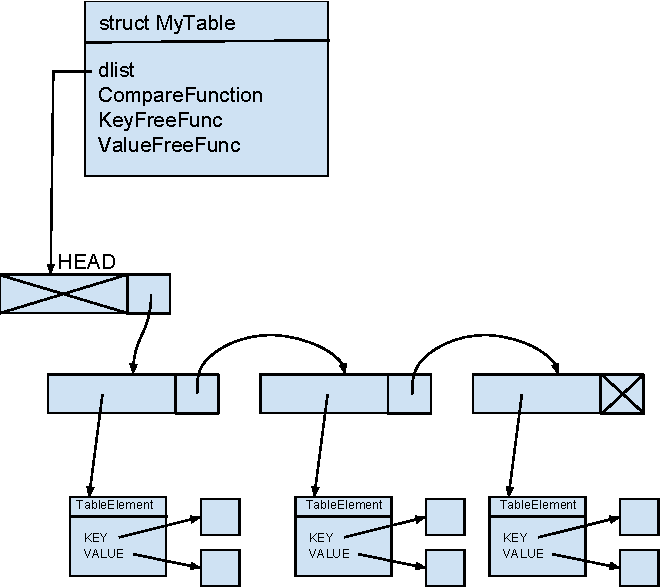
\includegraphics[width=0.7\textwidth]{figures/dlisttable.pdf}
\caption{\textit{Construction of the datatype dlist table and
    move-to-front list table.}}
\label{fig:dlisttable}
\end{figure}


\section{Material and Methods}
The description of the datatype `table' in the introduction applies to
the actual implementations which will be described below. A small
difference is that the coursebook \cite{janlert2000}, uses the wording
`argument' and `value' while the obtained implementation of a directed
list table uses the term `key' in the code.  
\subsection{Directed List Table and Move-to-Front List Table}
The structure of directed list table and move to front list table is
the same and can be seen in \textit{figure \ref{fig:dlisttable}}. The given
dlist was constructed with a `HEAD', using physical and logical
position where the physical is always one element before the logical. 
That means, when the requesting the content of the first
list element, the pointer is directed to `HEAD'. Then `head->next'
will be used to access the content of the first cell. This setup is
needed in a single directional list mostly for the `insert' operation:
The new element is inserted before the current element. If physical
and logical position would be the same, it would be needed to travers
the list again up to the position where the new element shall be inserted
and array table implementation but also of the given directed list.

The special feature about the move-to-front list table is the lookup
operation: each time, an element is looked up, it is moved to the
front of the directed list. A schematic of this operation can be seen
in \textit{figure \ref{fig:movetofront}}. The arrows in black show the
initial situation and the red arrows new situation after moving the
looked up cell to the front. In \textit{figure \ref{fig:movetofront}},
the cell to be moved to the front is the one in the middle.

The request to remove a non-exisiting key results in both the given
directed list table and the move to front list table in a traversal 
of the whole list, altough without any feedback. In case of duplicate
key values on an insertion, the old key/value pair is overwritten. In
more abstract terms, duplicates are handled at insertion time. 

\begin{figure}[H]
\centering
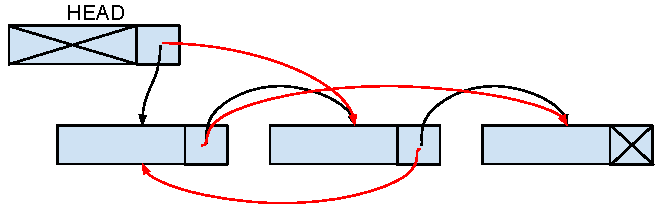
\includegraphics[width=0.5\textwidth]{figures/movetofront.pdf}
\caption{\textit{move to front operation in a directed list.}}
\label{fig:movetofront}
\end{figure}



\subsection{Array Table}
The structure of the array table can be seen in \textit{figure
  \ref{fig:arraytable}}. Instead of the directed list it is now
an array of void pointers. The table is initialized to NULL
pointers. On insertions, the void pointers of the array field is then
set to point to the new table element. The current implementation
traverses the array from low to high until an array field with NULL
pointer or the same key as the one to insert is found. On removal
of a key/value pair, the whole array is traversed to discard eventual
duplicate key entries. In more abstract terms, duplicates are handled
partly at insertion time and partly but definite at removal time. 
If a non-existing key is given as argument to
the remove operation, the whole array will be traversed. In the
current implementation no feedback is given whether a key was found
and removed or not.   

An important feature to mention is that by definition an array is a 
static datatype while a table is dynamic. This will be discussed in 
more detail. Also by definition, they index of an array is usually a 
natural number or integer which does not match with the definition of 
the argument/key in a table. A direct mapping from argument/key to 
array index is therefore in the most general case not possible. 


\begin{figure}[H]
\centering
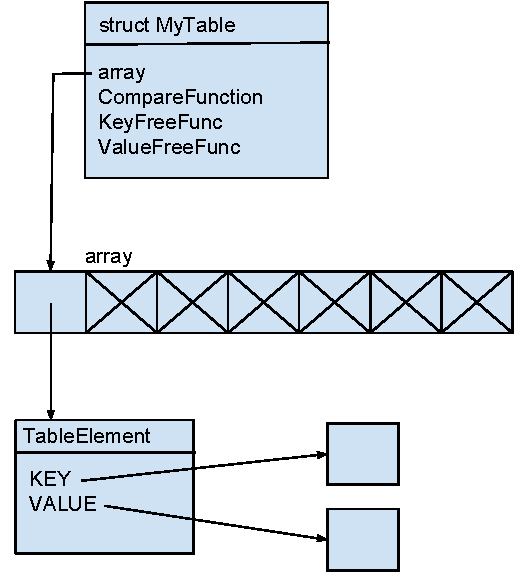
\includegraphics[width=0.5\textwidth]{figures/arraytable.pdf}
\caption{\textit{Construction of the array table data type.}}
\label{fig:arraytable}
\end{figure}

\subsection{Proposed changes to the interface}
Currently, the interface specification does not implement any 
return value for the operations `remove',`insert' and `free'. For
those three, a boolean feedback whether the operation succeeded would
certainly make sense. This would for example provide the information
whether a key requested for removal was available in the table or
not. For the `insert' operation, it could provide a signal in the
table array implementation when the underlying array is full with
values. 


\section{Results}
\subsection{Correctness of datatype implementations}
Two assess the correctness of the implemented datatypes a set of eight
tests was provided:

Correctness of the data types was assessed by eight
\begin{itemize}
\item `isEmtpy' on a new created table yields TRUE
\item insert a single element
\item lookup a single element
\item insert and lookup multiple elements with non identical keys
table
\item insert and lookup multiple elements with identical keys
\item remove a single element
\item remove elements with different keys
\item remove elements with the same key
\end{itemize}

The tests follow to a large extent the axiomatic table defintion given
in the course book \cite[p 122]{janlert2000}. All the implemented
tables fulfilled the test criteria.

\subsection{Performance tests}
The performance of the implemnted datatypes was asses by five
different tests that represent typical operations and use cases for
the datatype table. 

\begin{itemize}
\item Insertion speed
\item random existing lookup speed
\item random non-existing lookup speed 
\item skewed lookup speed
\item remove speed  
\end{itemize}

All above mentioned tests took as parameter the number \textit {n} 
of operations to be run for each separate test. This allows to assess the
time-complexity when performing the test for a series of increasing
\textit{n}. The test data generation procedure was also provided and
was based on the C `rand' function. To account for worst/best case
scenarios stemming from the random numbers, each test was run 10
times. Results below are presented as scatter plots (a) with
arithmetic means of ten runs for each \textit{n} operations case. 
The (b) plots show the relative standard deviation (RSD) for the 10
replicate runs in each \textit{n} operations point.  



\begin{figure}[H] 
\centering 
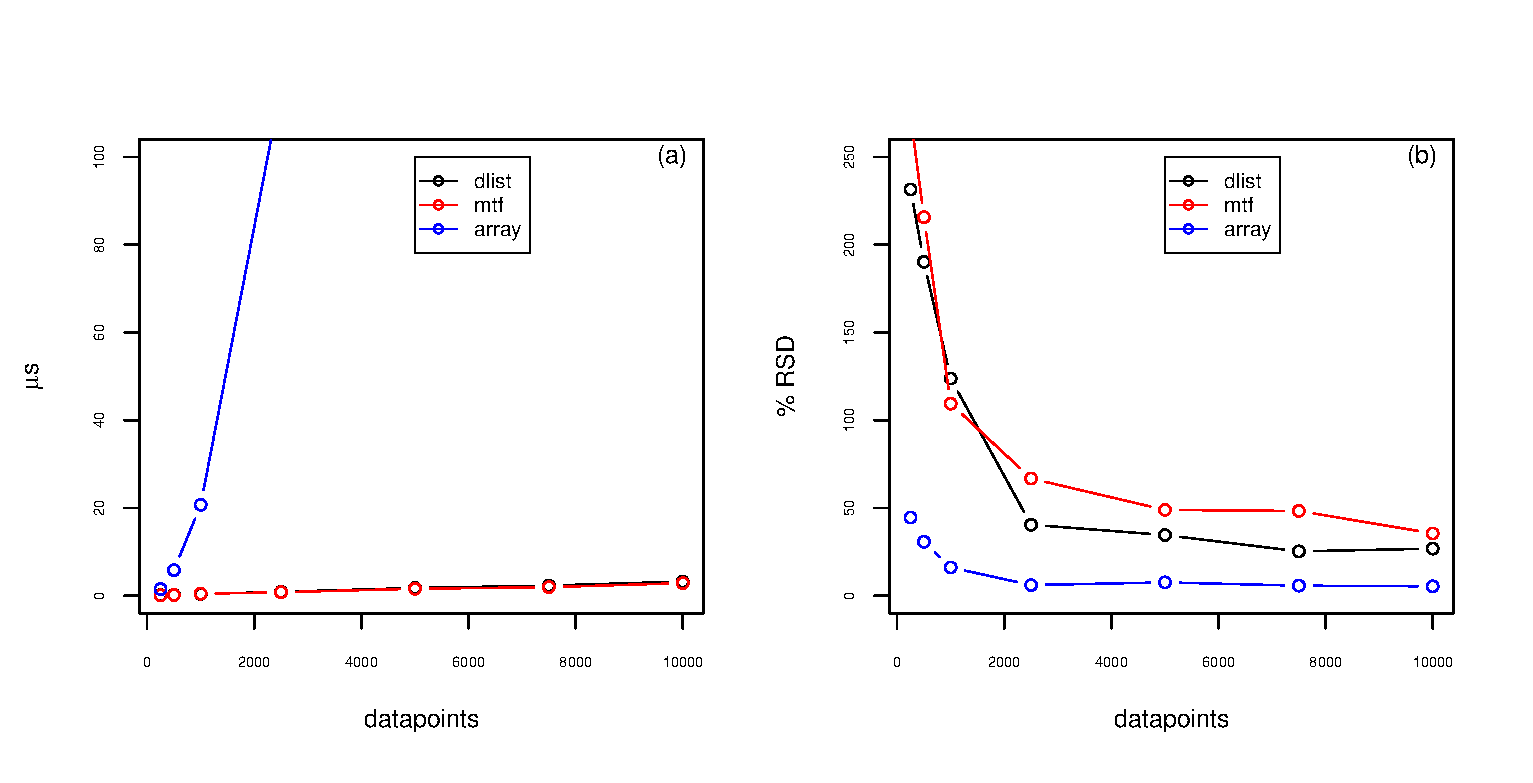
\includegraphics[width=\textwidth]{figures/fig1.eps}
\caption{\textit{Figure 1a, shows the element \textbf{`insertion'}
    times. Figure 1b shows the RSDs from the measurments in figure 1a. n=10.}}
\end{figure}

\begin{figure}[H] 
\centering 
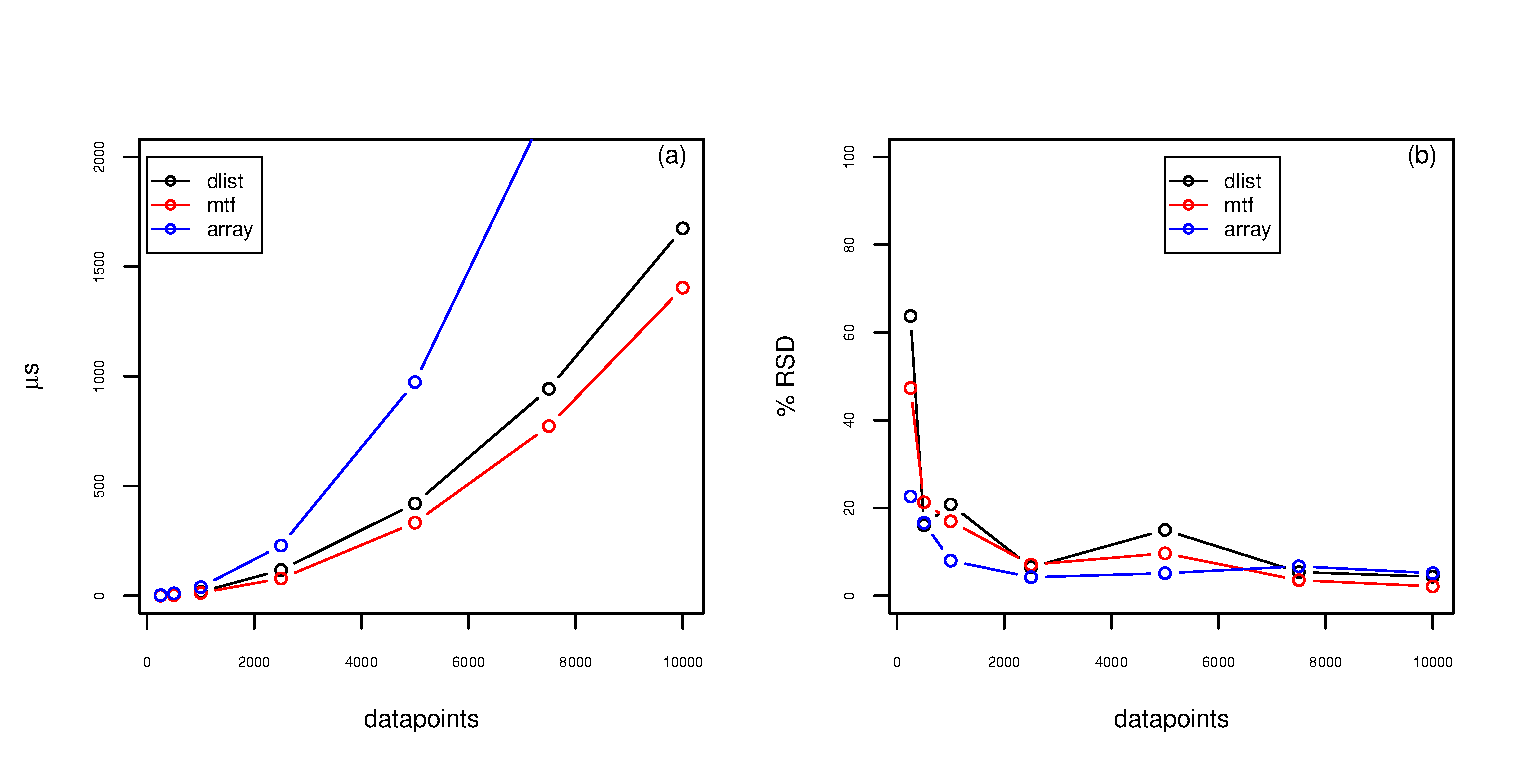
\includegraphics[width=\textwidth]{figures/fig2.eps}
\caption{\textit{Figure 2a, shows the times for the \textbf{`Random Existing
    Lookup'} benchmark. Figure 2b shows the RSD's from the measurments
in figure 2a. n=10.}}
\end{figure}

\begin{figure}[H] 
\centering 
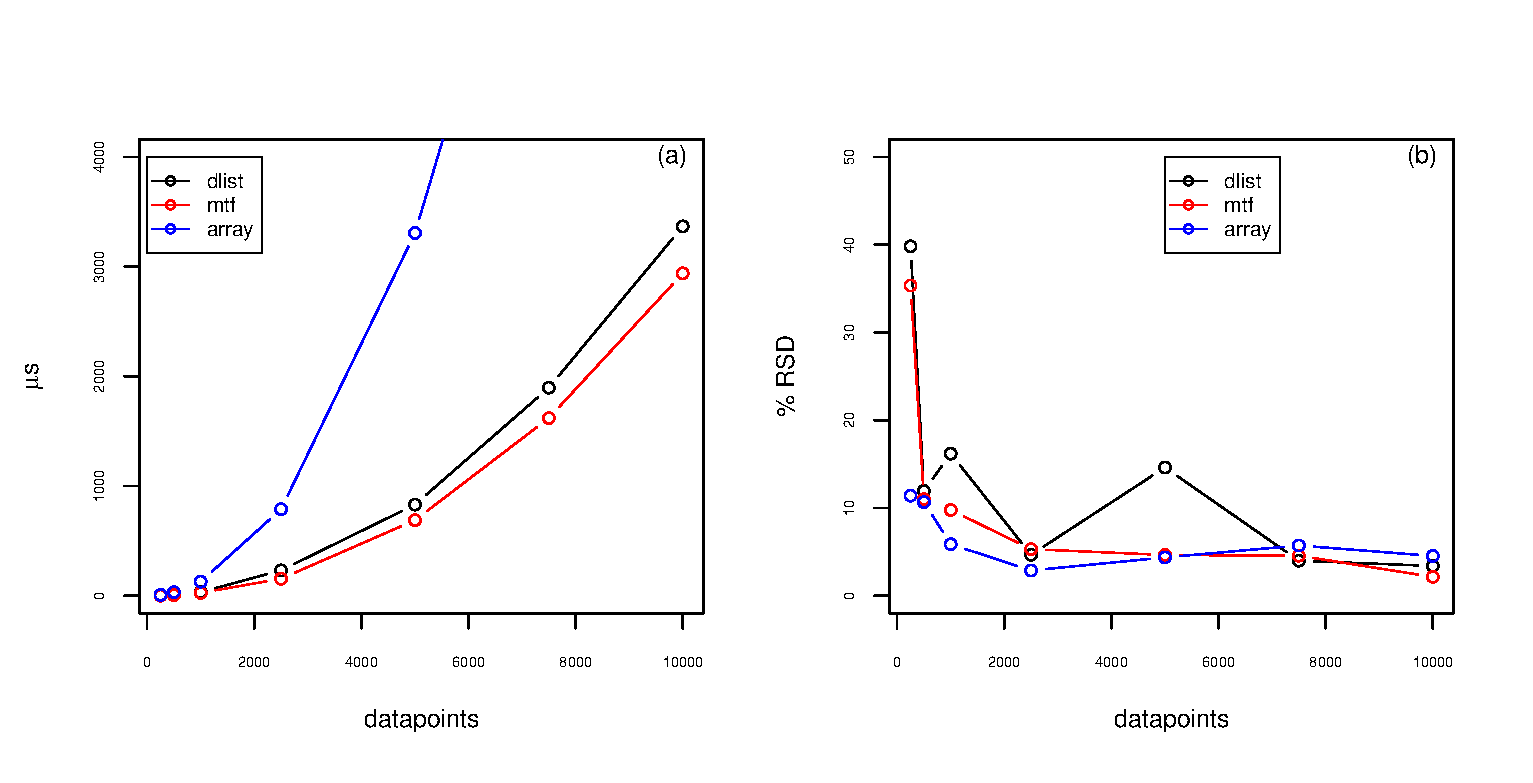
\includegraphics[width=\textwidth]{figures/fig3.eps}
\caption{\textit{Figure 3a, shows the times for the \textbf{`Random
      Non-Existing Lookup'} benchmark. Figure 3b shows the RSD's from
    the measurments in figure 3a. n=10.}}
\end{figure}

\begin{figure}[H] 
\centering 
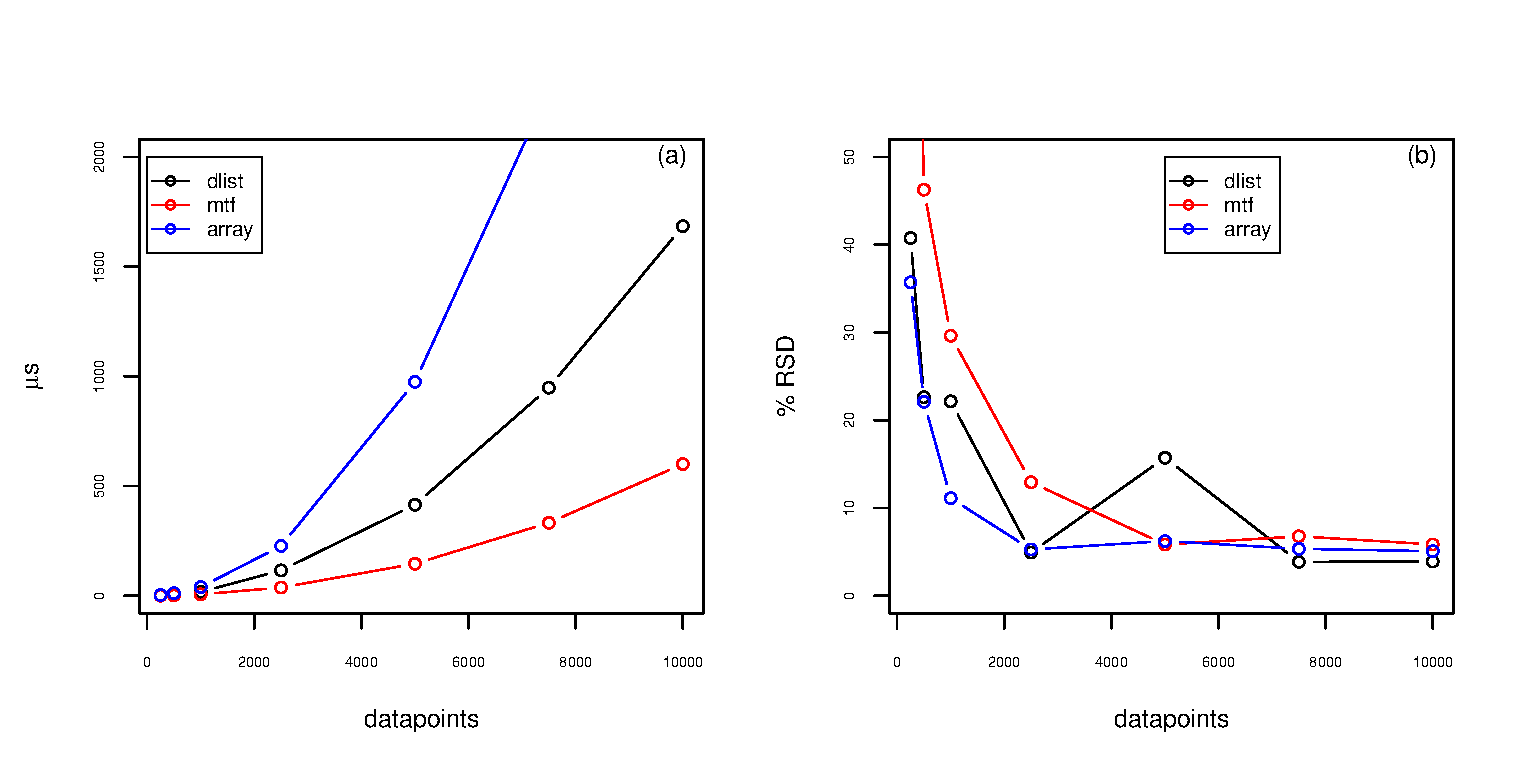
\includegraphics[width=\textwidth]{figures/fig4.eps}
\caption{\textit{Figure 4a, shows the times for the \textbf{`Skewed
      Lookup'} benchmark. Figure 4b shows the RSD's from the
    measurments in figure 4a. n=10.}}
\end{figure}

\begin{figure}[H] 
\centering 
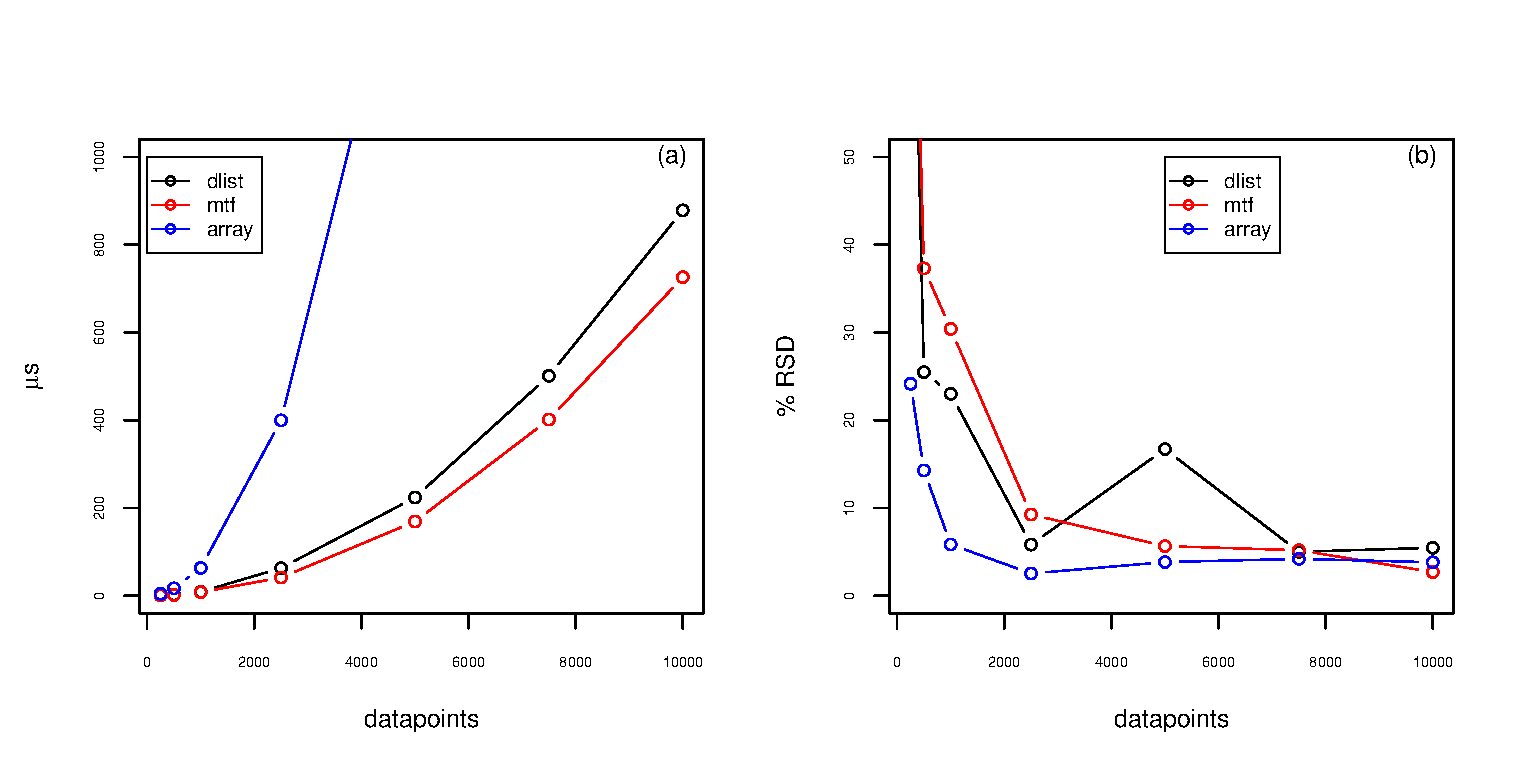
\includegraphics[width=\textwidth]{figures/fig5.eps}
\caption{\textit{Figure 5a, shows the times for the \textbf{`Removal'}
    benchmark. Figure 5b shows the RSD's from the measurments in figure 5a. n=10.}}
\end{figure}

\begin{figure}[H] 
\centering 
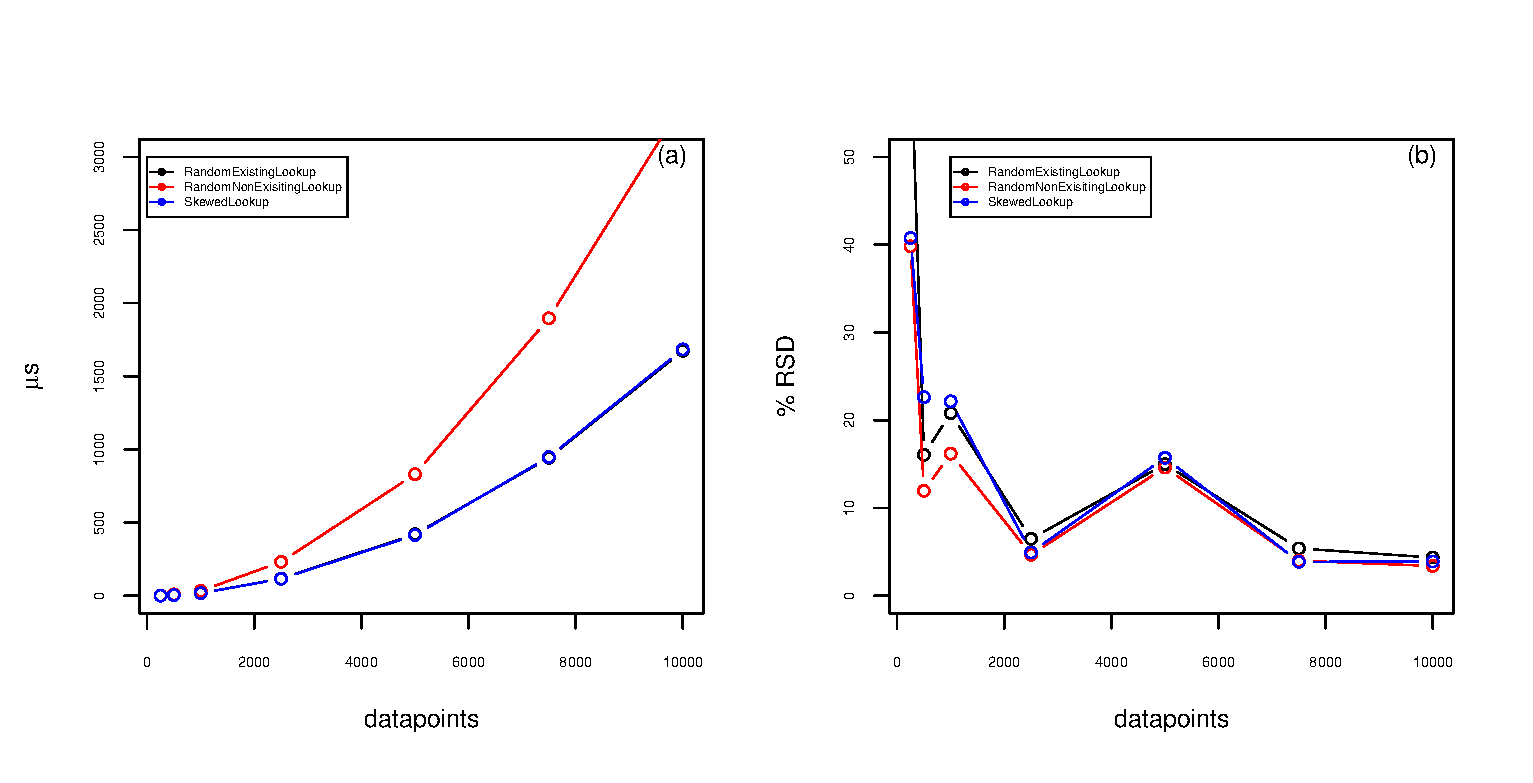
\includegraphics[width=\textwidth]{figures/fig6.eps}
\caption{\textit{Figure 6a, shows the times for the \textbf{`Random Existing
    Lookup'}, \textbf{`Random Non-Exisiting Lookup'} and
  \textbf{`Skewed Lookup'} benchmark of the datatype \textbf{`dlist'}. Figure 6b shows the RSD's from the measurments
in figure 6a. n=10.}}
\end{figure}

\begin{figure}[H] 
\centering 
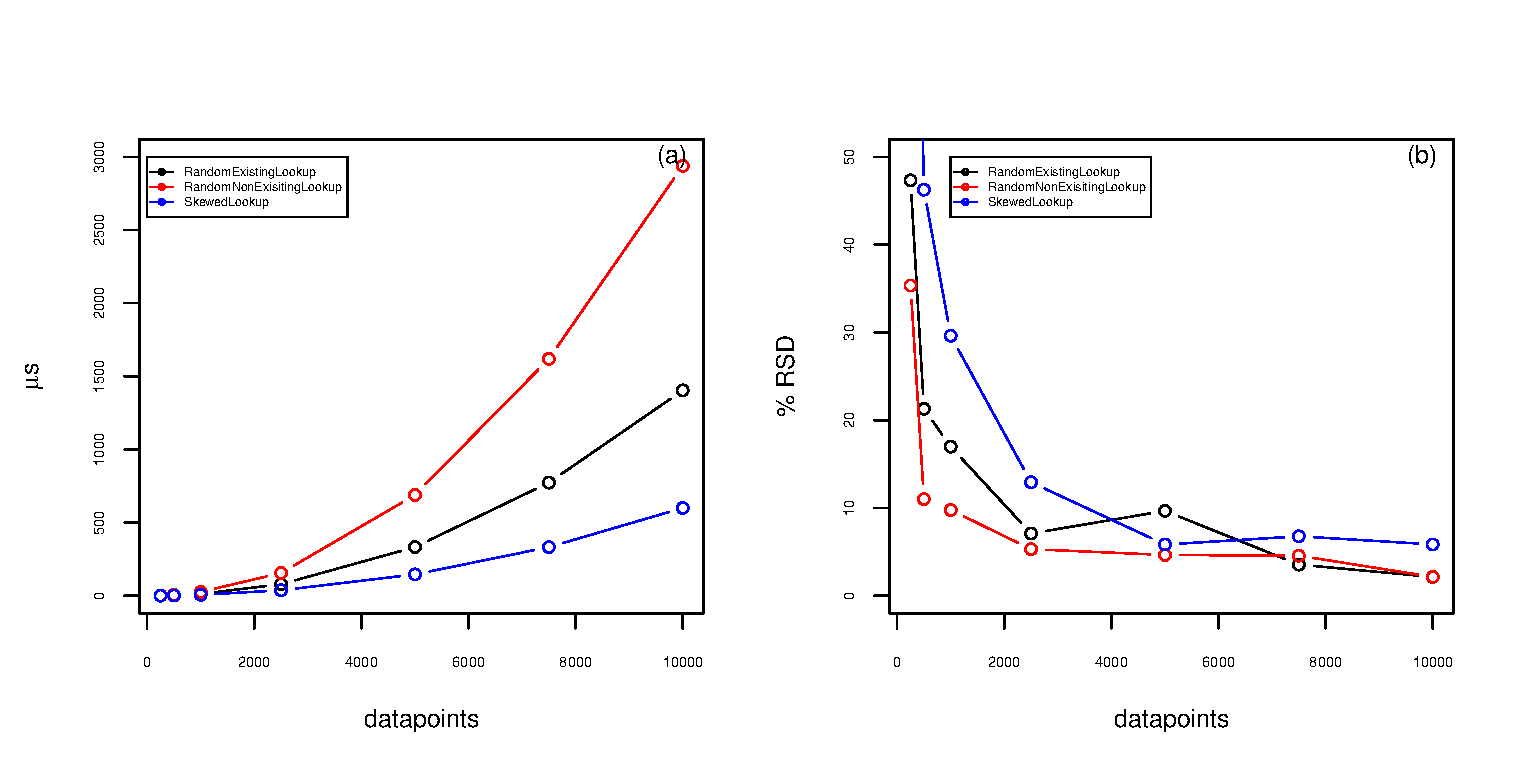
\includegraphics[width=\textwidth]{figures/fig7.eps}
\caption{\textit{Figure 7a, shows the times for the \textbf{`Random Existing
    Lookup'}, \textbf{`Random Non-Exisiting Lookup'} and
  \textbf{`Skewed Lookup'} benchmark of the datatype \textbf{`mtf'}. Figure 7b shows the RSD's from the measurments
in figure 7a. n=10.}}
\end{figure}

\begin{figure}[H] 
\centering 
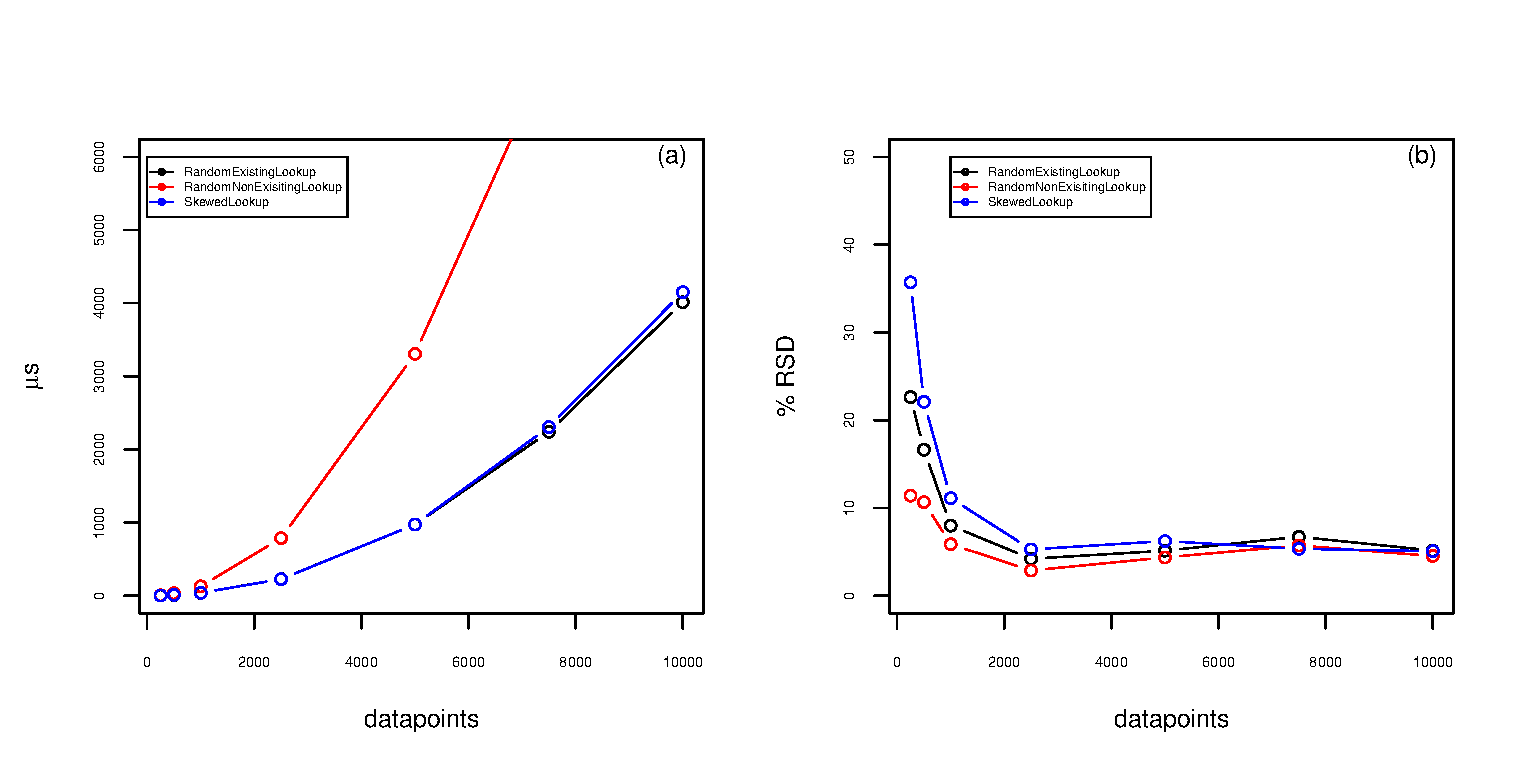
\includegraphics[width=\textwidth]{figures/fig8.eps}
\caption{\textit{Figure 8a, shows the times for the \textbf{`Random Existing
    Lookup'}, \textbf{`Random Non-Exisiting Lookup'} and
  \textbf{`Skewed Lookup'} benchmark of the datatype \textbf{`array'}. Figure 8b shows the RSD's from the measurments
in figure 8a. n=10.}}
\end{figure}


\section{Discussion}
Analysis of the results (1-3 pages). Flowing text. Shall answer at
least the following questions:
Which datatype was fastest, which (dis)advantages do the different
tabeltypes have? Reason for one advantage why the other implementation
don't offer it. Reasoning about dynamic/static implementation. If
done, reason why the direct indexing table is so fast.

\addcontentsline{toc}{section}{\refname}
\bibliography{references}

\end{document}
